\section{Techniques for Channel Sounding}
\label{sec_sounding_techniques}

Methods and systems for evaluating \ac{MU-MIMO} transmissions have evolved over the years as the \ac{WURC} platform matured as has our understanding of the logistical and signal processing complexities of large-scale \ac{MU-MIMO} beamforming on an \ac{SDR} platform.

In this section, we present the methods and systems used for the channel sounding experiments presented in this chapter, building from narrowband \ac{MU-MIMO} channel estimation for \textit{static} \acp{STA} all the way to a wideband, real-time channel sounding systems supporting completely \textit{mobile} \acp{STA}.


%\subsection{Mobile Signal Strength Mapping (Wardriving)}
%\label{sec_wardrive_technique}
	%
	%\rgnote{Hacked Atheros driver and frequency translation wardriving method: GPS puck and tagged packet receptions -- no channel estimates are available from the hardware, though}

%#################################################
\subsection{Static Single-Carrier Sounding}
\label{sec_static_miso_mubf}

	One of the primary reasons to develop the WARPLab platform integrations in Section~\ref{sec_warplab} was to be able to plan and execute multi-user channel sounding experiments with over-the-air multi-user beamforming in real-world scenarios.
	
	Consider a 4x2 system performing a downlink transmission where we wish to estimate the downlink beamformed \ac{SINR} from a 4-radio \ac{AP} to two \acp{STA}.
	Ideally, the linear pre-coder would eliminate interference from each spatial stream to each unintended receiver; however, we know that channel estimation errors and receiver spatial separation potentially increase the inter-user interference and would like to measure this effect in real environments.
	
	We employ a WARPLab-based MU-MIMO framework that is based on directly estimating the channel \ac{SINR} in its constituent terms and then computing the Shannon capacity to estimate the achievable rate of a transmission system.
	This is accomplished by a single-carrier measurement technique adapted from \cite{aryafar2010design} and shown in Fig.~\ref{fig_exTrans}.
	Here, the transmitter \ac{AP} beamforms sections of the transmission packet independently to accurately measure the SINR at the \acp{STA}.

\begin{figure}[ht]
\centering
  	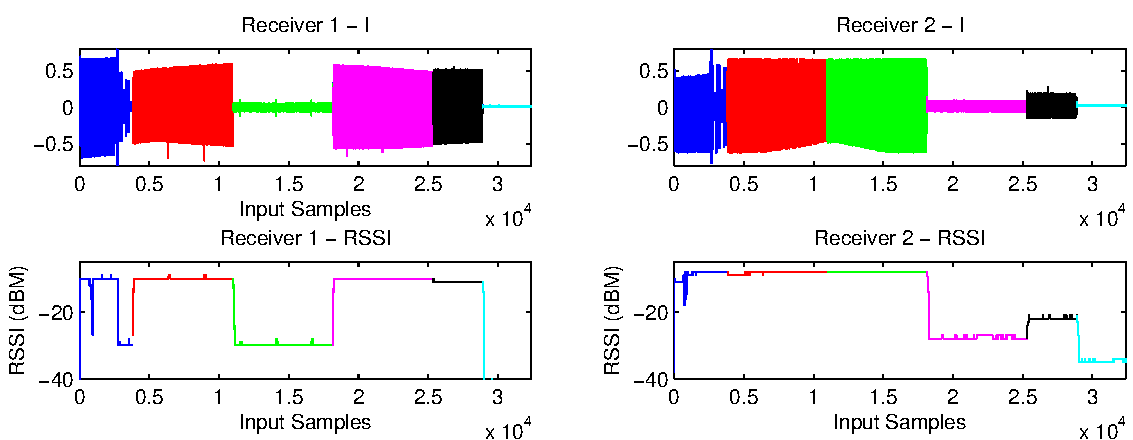
\includegraphics[width=6in]{figs/exTrans}   
   	\caption{Example RSSI Measurement used in achievable capacity calculation.
	\label{fig_exTrans}}
\end{figure}

	In the depicted 4x2 transmission example, the transmitter first sends an 802.11 \ac{STF} and \ac{LTF} preamble for gain control and timing synchronization (blue) and then performs a MU-MIMO transmission to both users (red).
	In the following two sections (green, purple), the transmitter sequentially zeroes out the data stream to each receiver individually in order to measure noise and interference at each receiver during the \ac{MU-MIMO} transmission.
	In the example 4x2 case, this becomes a single-user beamformed transmission, however in the 4x3 or 4x4 case, two or three receivers would be beamformed to during this measurement.

	Thus, the difference between the full MU-MIMO transmission containing both signal, noise, and interference at each receiver (red) and the transmission containing just interference and noise at the zeroed-out receiver (green or purple) is each transmitter's SINR.
	From there, we can compute aggregate Shannon Capacity as $C=log_2(1+\text{SINR})$.

	This method is quite effective to obtain an estimate for the multi-user interference in a downlink \ac{MU-MIMO} transmission, however it does have one drawback aside from the time required for cycling through different transmission modes.% and obtaining a statistically significant number of samples to estimate \ac{RSSI}.
	Since it directly measures channel noise power during a silent period, it is possible that the noise power estimation is amplified since it measures both channel noise and receiver noise simultaneously.
	Most of the time, the interference term will dominate noise floor in \ac{SINR} and this would not matter, but in highly-separable channels, it is possible that the channel noise will be smaller than the receiver thermal noise and this method will underestimate the channel quality.


%#################################################
\subsection{Static 802.11 Channel Sounding}
\label{sec_static_miso_chan_est}

	While the single-carrier system is useful for performing narrowband experiments, 802.11af is a wideband protocol utilizing channel bandwidths up to 32~MHz wide \cite{flores2013ieee80211af}.
	In addition, UHF channels have reported empirical indoor 0.9 coherence bandwidth between 6-16~MHz \cite{varela2001rms} and empirical outdoor urban/suburban 0.5 coherence bandwidth on the order of 0.5-2~MHz \cite{bajwa1985large}.
	Additional experimental results have indicated very small resolution channel estimation on the order of 19.5~kHz may be relevant for signal processing in \ac{TVWS} systems \cite{zhang2016watch}.
	All together, this means that we wish to obtain channel state information and perform beamforming at a small granularity across the wide 802.11af channel bandwidths to be sure to capture UHF channel dynamics.

	%Luckily, our implementation of a real-time 802.11af-like stack implements a real-time layer-2 wireless bridge utilizing an 802.11a/g AP and STA design with a completely open network stack.
	To perform wideband channel sounding to multiple user \acp{STA}, the real-time capabilities of the 802.11 reference design are leveraged to provide fine-grained continuous channel estimates from multiple transmitting antennas in order to directly measure the \ac{MU-MIMO} channel capacity instantaneously and over a long period of time.

	The legacy 802.11 design calculates and stores channel state information as required by its OFDM channel equalizers, however, this information is generally discarded after packet reception.
	The channel estimation extracted from each received 802.11 PLCP header \cite{std11ac} provides a complete \ac{CSI} estimation matrix that can be used as a single-antenna sounding event.
	We modify the physical layer of the WARP 802.11 Reference Design \cite{warp80211} to treat each of a series of transmitted PLCP headers as separate ``packets'' for the purpose of \ac{CSI} measurement from multiple transmitting antennas.

	Our custom sounding ``packet'' is a brief 802.11g-like signal containing PLCP header for packet detection, AGC convergence, and symbol timing extraction.
	The payload is just long enough to provide error detection bits and identifying information about the transmitter so that the transmitting antenna can be identified.
	Due to the small size of this sounding packet, it is not compliant with the requirement that 802.11 packets contain an 802.11 and link-layer header.
	Therefore, we modify the MAC software to pass all packets regardless of valid header or fields to the Ethernet interface for processing.
	
	\begin{figure}[htb]
\centering
  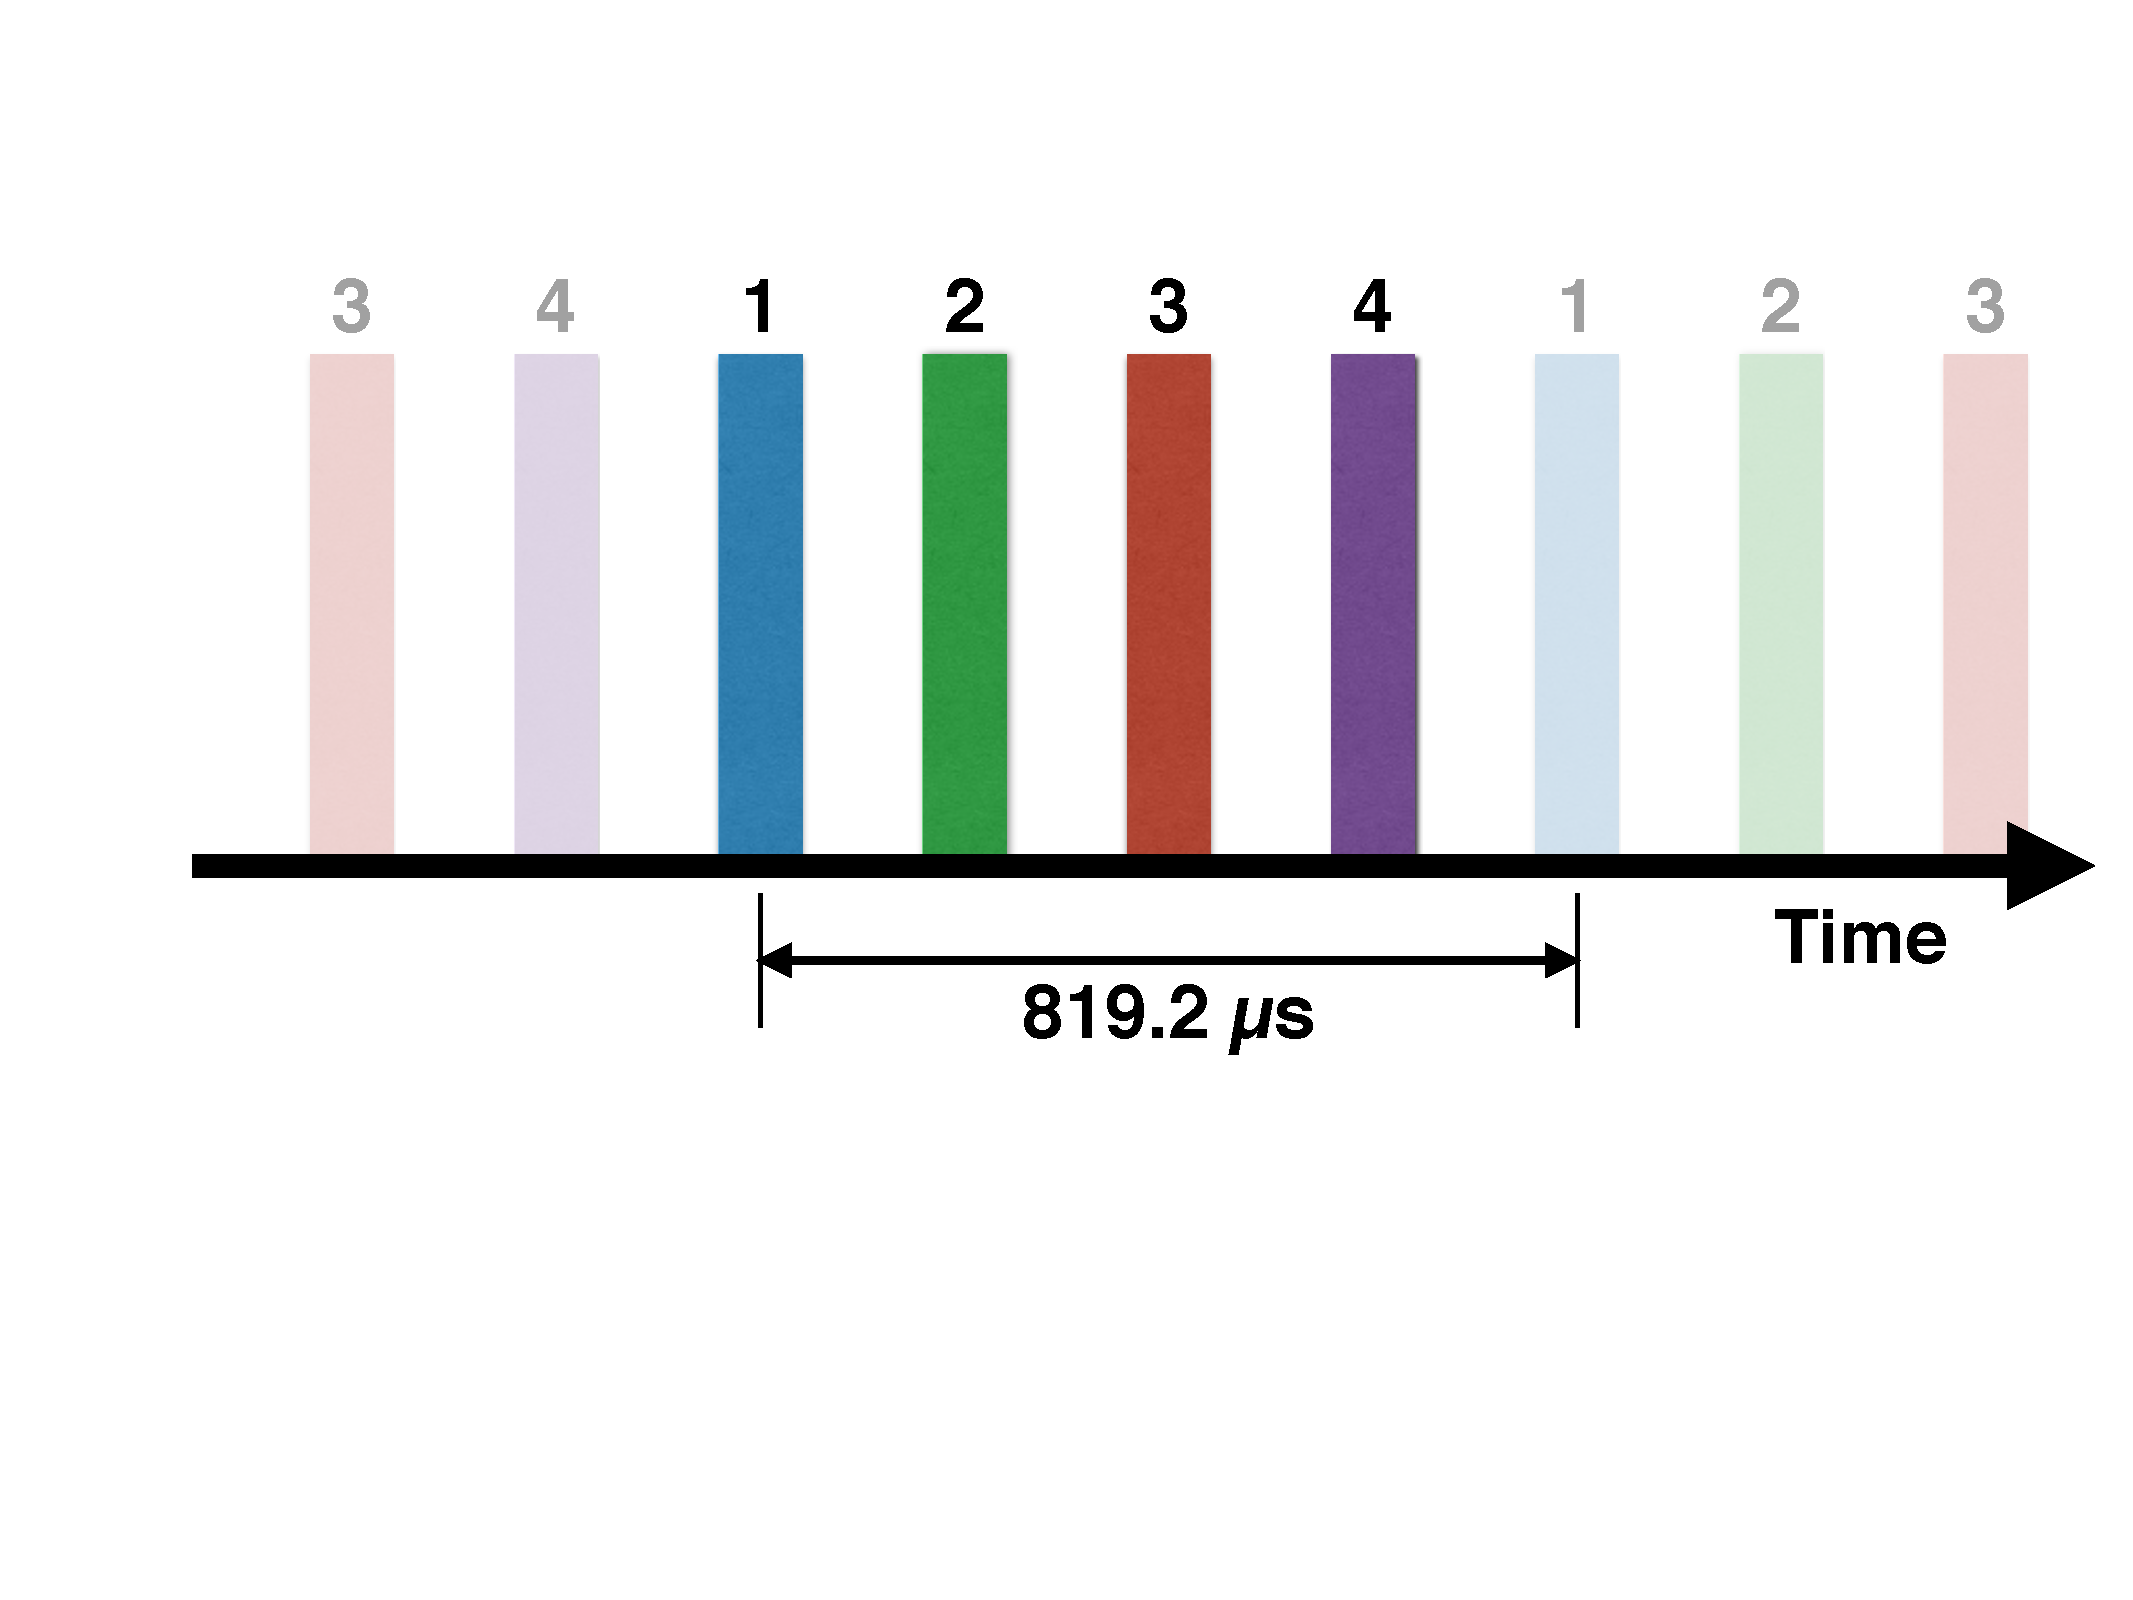
\includegraphics[width=2.7in]{figs/ryan_sounding_example}   
    \caption{Short timing packets are sent from each of the \ac{WURC} array antennas in rapid succession consisting of an 802.11 PLCP preamble and a short, 14-byte payload.}\label{fig:sounding}
\end{figure}

	We construct this special sounding packet in MATLAB and preconfigure the \ac{WURC} array, running our WARPLab modification, to transmit these packets continuously staggered in time as shown in Figure \ref{fig:sounding}.
	Tests show that WARPLab continuous-transmit mode remains synchronous over long periods of time if the boards are clock synchronized.
	We provide sufficient spacing between sounding packets to allow the 802.11 PHY to process the previous packet and reset, and we find that the WARPLab buffer size of 32768 samples over 819.2~$\mu s$ is sufficient to capture channel variation even at higher frequencies.

We combine this structure with a set of multiple listening nodes that process these channel sounding packets and can then store them for later retrieval.
A ten-minute packet trace for a single antenna can run over 1 GB in size, so substantial buffering and disk I/O speed is required for the recording nodes.
	
%#################################################
\subsection{Static 802.11 MU-MIMO Beamforming}
\label{sec_static_beamforming}

	We wish to perform the same type of multi-user beamformed channel estimation as in Section~\ref{sec_static_miso_mubf}, except modified for wideband channel sounding.

	A fundamental tradeoff of \ac{SDR} equipment is that one generally sacrifices processing speed for the sake of flexibility, which becomes a problem when performing closed-loop beamforming operations where performance can be severely degraded by processing delays and transmission latency.
	For this reason, very few published papers have attempted to perform actual over-the-air beamformed transmissions, opting instead to post-process and \emph{estimate} beamforming performance from channels estimated in both uplink and downlink directions.

	Our approach to solving the processing delay in \ac{SDR} equipment is to take advantage of the higher coherence time of low-frequency channels and perform over-the-air experiments on selected UHF (470-698~MHz) channels, where the processing latency becomes much less significant.
	We will show in Chapter~\ref{sec_environment_chapter} that this approach is suitable to the longer channel coherence times and reduced sensitivity to user mobility.

	To this end, we implement a beamforming and channel-sounding framework based around the 802.11af WiFi standard, in order to compare against 2.4/5~GHz implementations of 802.11ac since the physical \ac{OFDM} layers of 802.11ac VHT 40~MHz and 802.11af TVHT 5~MHz are identical aside from the radio sampling rate \cite{std11af,std11ac} \cite{guerra2018toolbox}.
	
	Standards-compliant piloted phase correction is implemented to compensate for sample timing drift during the payload, necessary to yield accurate measurements of received \ac{EVM}.
	Two copies of the cyclicly-shifted L-STF provide ample time to account for AGC settling and the WARPLab trigger jitter.
	Timing recovery and carrier-frequency offset correction operates on the L-LTF field, while we utilize the TVHT-LTF symbols with the 802.11af spatial spreading matrix for channel estimation.
	
%\rgnote{This is where the development work for Uri's experimental paper goes. I basically implemented MATLAB's 802.11ac toolbox on WARP/WURC before it was a toolbox. As a personal, note, this was a significant development contribution, but I ended up not using it for any experimental study. Based on what I learned building the system and attempting to implement implicit calibration, I decided to move on to a complete system redesign (IRIS and ``Argos''). However, this work was used in currently submitted CSI security work that was led by Uri and also Naren.}

%#########
\subsubsection{Multi-Stream Noise and Channel Estimate}
\label{sec_static_mubf_chan_est}

	Our analysis requires updated \ac{CSI} for each downlink beamformed packet as well as \ac{CSI} noise variance.
	To provide these measurement metrics, we take two approaches depending on the transmission direction and number of streams.

% WURCLab multi-stream bemformed channel sounding with ground truth
\begin{figure}[ht] 
\centering
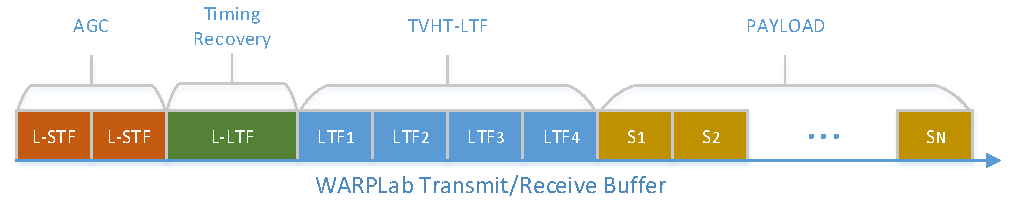
\includegraphics[width=1\linewidth]{./figs/packet_format.pdf}
\caption{Multi-stream beamformed packet format implements the 802.11af TVHT 5~MHz PHY, utilizing the TVHT-LTF for multi-stream channel sounding.}
\label{fig:packet_format}
\end{figure}

	On the multi-stream downlink beamformed packet, we send an extra \textit{non-beamformed} TVHT-LTF (blue) immediately following the beamformed TVHT-LTF (green) as shown in the timing diagram in Figure~\ref{fig:packet_format}.
	
		In the case where power is allocated equally across receivers, each transmit antenna has the same transmit power budget, and the channel is \emph{i.i.d.} Rayleigh, the per-user expected beamformed \ac{SINR} can be expressed \cite{anandpuma} as
\begin{equation} \label{eq_expected_bf_sinr}
\mathcal{E}\{ SINR\} = 10\cdot \log_{10}\bigg( \frac{M-K+1}{K}\frac{(P/N_O)}{M} \bigg).
\end{equation}
	This approximation, valid for environments with rich multipath, provides a power scaling factor for the non-beamformed \ac{LTF} fields that allows a receiver that has performed \ac{AGC} on the beamformed \ac{STF} (orange) in Figure~\ref{fig:packet_format} to also resolve non-beamformed signals.
	
	When scaled according to the expected degradation in beamformed \ac{SNR} compared to broadcast \ac{SNR} \cite{anandpuma} to avoid \ac{AGC} clipping, this extra TVHT-LTF provides an estimate of the multi-user wireless channel \emph{at the exact moment} that the beamformed packet is sent.

	On the single-stream uplink channel, we assume that the wireless channel is constant for the WARPLab buffer, then we can apply the noise variance estimation technique developed in \cite{ren2009snr} to estimate the packet noise variance \ac{SNR}. 
	The same estimator may be used for the individual zero-forced streams of the multi-stream downlink packet.
	
	The end-to-end latency of a sound-precode-transmit operation on our \ac{WURC} array using WARPLab 7.4 ranges from 71~ms for a $4\times 1$ transmission to 173~ms for a $4\times 4$.
	This approach of operating on UHF channels is validated in that we are consistently able to achieve less than 5\% receive \ac{EVM} at 16-QAM in an office environment with $4\times 2$ \ac{MU-MIMO}, provided the \acp{STA} are static.
	
	%The MATLAB library developed for this is released open-source for use on WARPv3 or WARPv3 platforms \cite{guerra2018toolbox}.
	
	
%#################################################
\subsection{Mobile Measurement System: Rapid Implicit Sounding}
\label{sec_mobile_chan_est}

 Channel sounding of mobile devices has always presented a challenge for \ac{SDR} systems, which require extensive computational resources, power sources, and  synchronization to operate as a stand-alone mobile device.
 For that reason, our early multi-user UHF research focused solely on fixed devices \cite{anand2014case} and avoided investigations of channels with nodal mobility.

	As \ac{MU-MIMO} channel sounding techniques advanced, we once again leveraged the modular and compartmentalized design of \ac{WURC} and our driver libraries to port another \ac{SDR} framework to our platform in order to perform \emph{mobile} multi-user wide-band channel measurements.

 In order to sound the multi-user environment rapidly between a \ac{MU-MIMO} \ac{AP} and multiple mobile \acp{STA}, we ported the published Argos \ac{MU-MIMO} control channel \cite{shepard2015faros} to inter-operate with our new $8\times 8$ MIMO WURC array (Section~\ref{sec_wurc_8x8}) by integrating custom HDL and embedded C libraries for the WARPv3 platform. 
 The robust wireless synchronization scheme utilizing long correlatable signal sequences in Argos allows us to operate mobile \acp{STA} remotely, using a low-rate wireless side channel (the wireless bridge in Fig.~\ref{fig:wurc_argos_hw} for \ac{STA} initialization and control messages, while sample-level synchronization and implicit channel sounding occurs over the UHF channel.
 More details about the design of Argos are available in \cite{shepard2015faros}; we configure the system to allow us to sound the uplink channel of a set of mobile/static \acp{STA} every 2.5 to 5~ms.

	In order to increase the number of antennas available at the \ac{AP}, we share reference clocks between two $4\times4$ WURC \acp{AP} as discussed in Section~\ref{sec_wurc_4x4} to create a single $8\times8$ \ac{WURC} \ac{AP}.
	This significantly shortened clocking topology introduces no measurable decrease in signal or triggering error and has been validated over hours of operation. %, thus achieving our original design goals and providing new measurement capabilities in UHF bands.
	
	By starting from relatively simple narrowband channel sounding and building to wideband channel estimation as beamforming hardware and software support evolved, we developed a real-time multi-user and frequency-agile channel sounding system that allowed for true nodal mobility and could capture channel dynamics in small, millisecond packet timescales.
